\documentclass{ximera}


\graphicspath{
  {./}
  {ximeraTutorial/}
  {basicPhilosophy/}
}

\newcommand{\mooculus}{\textsf{\textbf{MOOC}\textnormal{\textsf{ULUS}}}}

\usepackage{tkz-euclide}\usepackage{tikz}
\usepackage{tikz-cd}
\usetikzlibrary{arrows}
\tikzset{>=stealth,commutative diagrams/.cd,
  arrow style=tikz,diagrams={>=stealth}} %% cool arrow head
\tikzset{shorten <>/.style={ shorten >=#1, shorten <=#1 } } %% allows shorter vectors

\usetikzlibrary{backgrounds} %% for boxes around graphs
\usetikzlibrary{shapes,positioning}  %% Clouds and stars
\usetikzlibrary{matrix} %% for matrix
\usepgfplotslibrary{polar} %% for polar plots
\usepgfplotslibrary{fillbetween} %% to shade area between curves in TikZ
\usetkzobj{all}
\usepackage[makeroom]{cancel} %% for strike outs
%\usepackage{mathtools} %% for pretty underbrace % Breaks Ximera
%\usepackage{multicol}
\usepackage{pgffor} %% required for integral for loops



%% http://tex.stackexchange.com/questions/66490/drawing-a-tikz-arc-specifying-the-center
%% Draws beach ball
\tikzset{pics/carc/.style args={#1:#2:#3}{code={\draw[pic actions] (#1:#3) arc(#1:#2:#3);}}}



\usepackage{array}
\setlength{\extrarowheight}{+.1cm}
\newdimen\digitwidth
\settowidth\digitwidth{9}
\def\divrule#1#2{
\noalign{\moveright#1\digitwidth
\vbox{\hrule width#2\digitwidth}}}






\DeclareMathOperator{\arccot}{arccot}
\DeclareMathOperator{\arcsec}{arcsec}
\DeclareMathOperator{\arccsc}{arccsc}

















%%This is to help with formatting on future title pages.
\newenvironment{sectionOutcomes}{}{}


\title{Periodic}

\begin{document}

\begin{abstract}
tides
\end{abstract}
\maketitle


The following data was collected recording the height of tides in Austraila (NSW Dept of Education).




\[
\begin{array}{ll}
\text{Time (hrs)}  & \text{Height (m)}  \\
0      &  1.63  \\
6.4    &  0.64  \\
12.2   &  1.36  \\
18.1   &  0.53  \\
24.9   &  1.69  \\
31.4   &  0.58  \\
37.1   &  1.32
\end{array}
\]


As expected, the heights seem to be periodic.  This suggests that a good model might be a sine or cosine function.  Since there seems to be a maximum height at time $0$, a cosine model is a good choice.




In the following DESMOS app, select choices for $A$, $B$, $C$, and $D$ to fit the model to the data.

\begin{center}
\desmos{9pmszixak2}{400}{300}
\end{center}


The best model is approximately

\[   H(t) = 0.495 \cos(0.515 t) 1.135       \]







\begin{image}
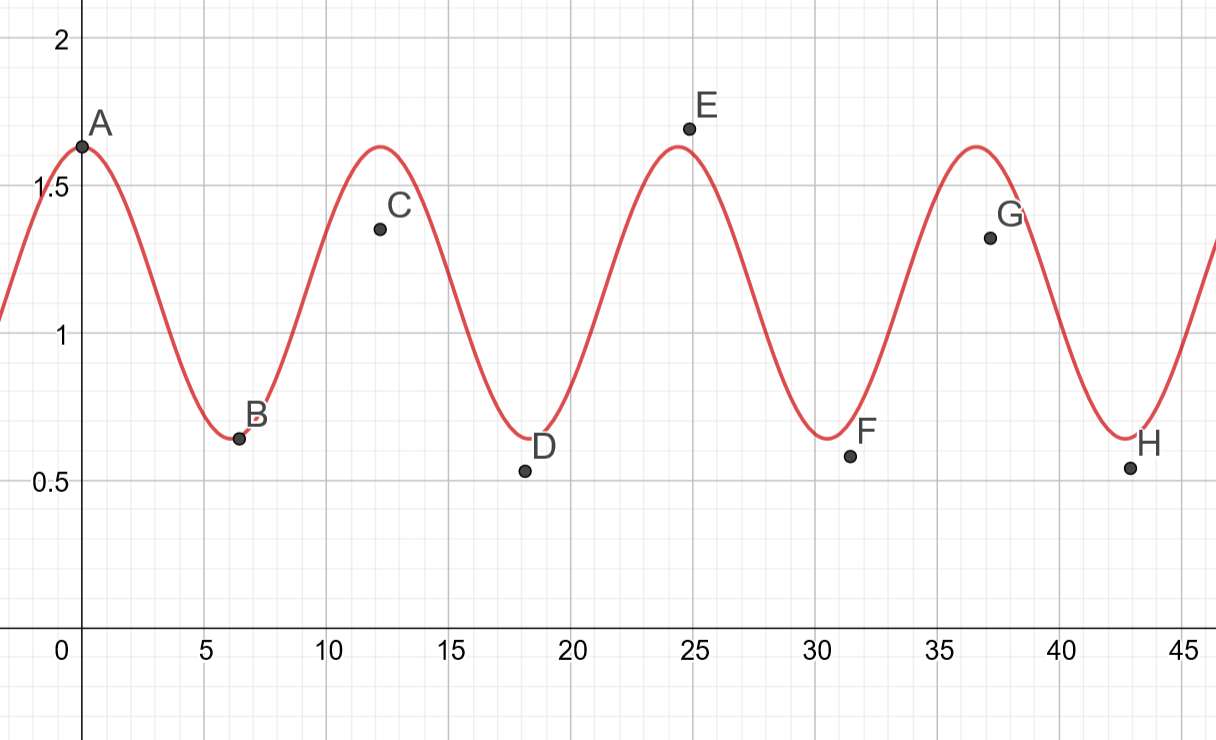
\includegraphics{pics/tides.png}
\end{image}


However, it doesn't do such a good job. It looks like every other high tide height is missed.\\


If we graph more of the data, we can see this better.





\begin{image}
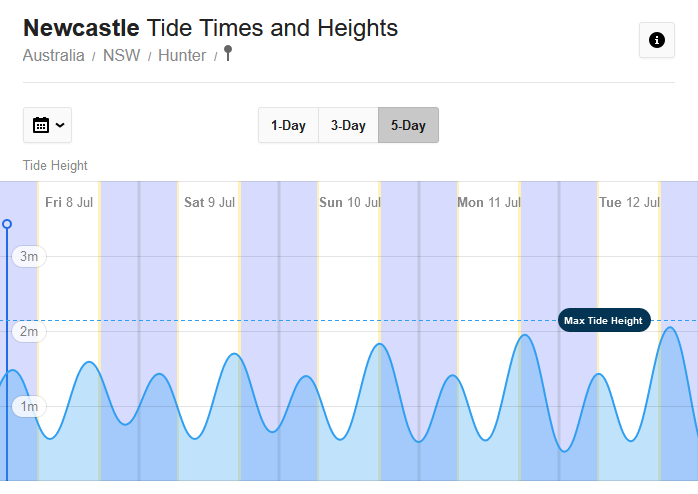
\includegraphics{pics/tides2.png}
\end{image}



There appear to be two sinusoidal waves of different heights.  \\

A better model might involve two cosine functions. \\


We need the model we have, but every other wave needs to be decreased a little bit.  Another cosine function with twice the period can do this. \\



When the model was a single cosine function, it appear that the period was approximately $12.2$ hours, which gives a frequency of $\frac{2 \pi}{12.2} = \frac{\pi}{6.1} = 0.515$, which was the coefficient inside the cosine function.  



\begin{question}  Period

If we switch the model to two cosine functions, then the period of the second cosine would be $\answer[tolerance=0.1]{24.4}$ hours.


\end{question}




\begin{question}  Period

If the period is $24.4$ hours, then the frequency is $\frac{2 \pi}{\answer{24.4}} = \frac{\pi}{\answer{12.2}}$.


\end{question}









Our new model begins to look like:

\[   H(t) = A \cos\left( \frac{\pi \, t}{6.1} \right) + B \cos\left( \frac{\pi \, t}{12.2} \right) + C       \]


We have three unknowns. \\

We need three data points. \\


We'll select the first three peaks/troughs:  $(0, 1.63)$, $(6.4, 0.64)$, and $(12.2, 1.36)$. \\



\textbf{\textcolor{blue!55!black}{$\blacktriangleright$}} $first(t) = \cos\left( \frac{\pi \, t}{6.1} \right)$ is the faster piece. \\


\textbf{\textcolor{blue!55!black}{$\blacktriangleright$}} $second(t) = \cos\left( \frac{\pi \, t}{12.2} \right)$ is the slower piece. \\




The second cosine function is slower funciton and has double the period as the first.  They both start at maximums at $t=0$.  Both functions have a value of $1$. \\

Then, the first cosine function arrive at its minimum of $-1$ at $t=0.64$, however, the second function is slower and is at a zero when $t=0.64$.  \\

At $12.2$ the first cosine is at it maximum of $1$ and the second function has arrived at its minimum of $-1$.






\begin{itemize}
\item At $(0, 1.63)$  we have $1.63 = A + B + C$
\item At$(6.4, 0.64)$ we have $0.64 = -A + C$
\item At $(12.2, 1.36)$  we have $1.36 = A - B + C$
\end{itemize}




From these three equations, we can see that $1.63 + 1.36 = 2 \, A + 2 \, C$   or $1.495 = A + C$.  \\

This and the second equation tell us that $0.64 + 1.495 = 2 \, C$ or $C = 1.068$. \\

We can put this in for $C$, in the second equation: $0.64 = -A + 1.068$ or $A = 0.4275$.

And, from all of this we get $B = 0.1345$.






\begin{center}
\desmos{ufauqfzfgk}{400}{300}
\end{center}

Much better.















\begin{center}
\textbf{\textcolor{green!50!black}{ooooo=-=-=-=-=-=-=-=-=-=-=-=-=ooOoo=-=-=-=-=-=-=-=-=-=-=-=-=ooooo}} \\

more examples can be found by following this link\\ \link[More Examples of Modeling]{https://ximera.osu.edu/csccmathematics/precalculus2/precalculus2/modeling/examples/exampleList}

\end{center}






\end{document}
